\section{Pregunta N$^{\circ}$5\qquad Andre Gilmer Santos Felix}

\begin{frame}
    \begin{enumerate}\setcounter{enumi}{4}
        \item


              Determine si la función
              \begin{math}
                  S\left(x\right)=
                  \begin{cases}
                      1+
                      x-
                      x^{3},                   & 0 \leq x<1      \\
                      1-
                      2\left(x-1\right)-
                      3{\left(x-1\right)}^{2}+
                      4{\left(x-1\right)}^{3}, & 1 \leq x<2      \\
                      4\left(x-2\right)+
                      9{\left(x-2\right)}^{2}-
                      3{\left(x-2\right)}^{3}, & 2 \leq x \leq 3
                  \end{cases}
              \end{math}
              es el spline cúbico natural que interpola en los puntos
              $\left(0,1\right)$, $\left(1,1\right)$, $\left(2,0\right)$ y
              $\left(4,10\right)$.
    \end{enumerate}

    \begin{solution}
        .
    \end{solution}
\end{frame}

\begin{frame}
    \begin{solution}
        \begin{figure}[ht!]
            \centering
            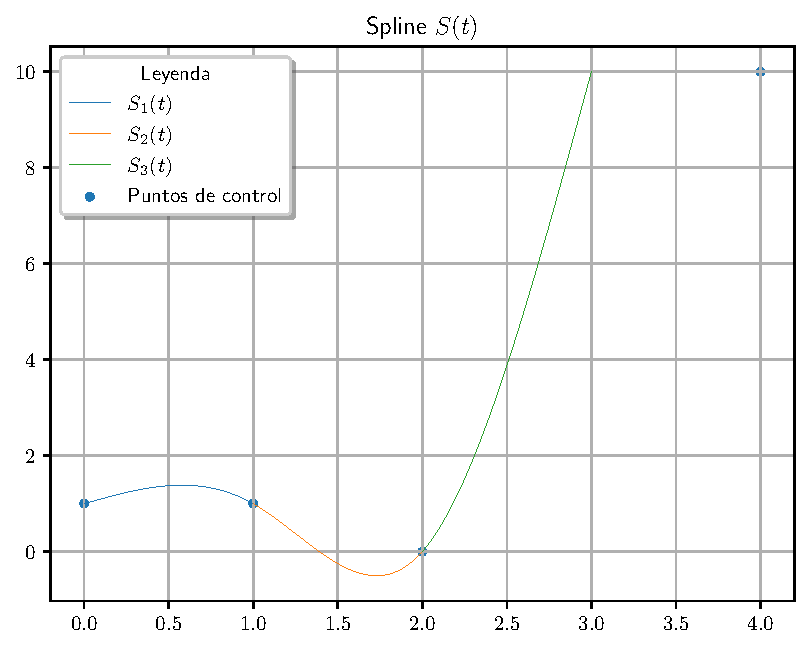
\includegraphics[width=.72\paperwidth]{p5}
        \end{figure}
    \end{solution}
\end{frame}